\documentclass[12pt]{article}

\usepackage[english]{babel}
\usepackage[utf8x]{inputenc}
\usepackage{pdfpages}
\usepackage{lastpage} % Required to determine the last page for the footer
\usepackage{extramarks} % Required for headers and footers
\usepackage{graphicx} % Required to insert images
\usepackage{listings} % Required for insertion of code
\usepackage{courier} % Required for the courier font
\usepackage{color}
\usepackage{grffile}
\usepackage{float}

\usepackage[a4paper, total={6in, 8in}]{geometry}

% Margins
\topmargin=-0.45in
\evensidemargin=0in
\oddsidemargin=0in
\textwidth=6.5in
\textheight=9.0in
\headsep=0.25in
\fboxsep=0mm%padding thickness
\fboxrule=2pt%border thickness

\linespread{1.1} % Line spacing

\newcommand{\Title}{Software Documentation Document} % Assignment title
\newcommand{\Class}{Cos\ 301} % Course/class
\newcommand{\pd}{Post-Doctoral}
\newcommand{\ssr}{Soft\color{green}{Serve }\color{black}}
\newcommand{\version}{0.9}
\newcommand{\iteration}{1}
\newcommand{\client}{Ms. Cathy Sandis (UP Research Office)}
\newcommand{\project}{Post-Doctoral Application Management System}

\begin{document}


\vspace{4em}

\begin{center}%

\begin{figure}[ht!]
\centering

\includegraphics{../Images_Docs/logo.png}
\end{figure}
\LARGE \bf \project \\[1em]
\LARGE \bf \Title \\[0.25em]
\large \bf \today\\
\bf Version \version\\
\bf Iteration \iteration\\[0.5em]
\Large \bf Prepared for \client\\
\Large \bf by
\Large {\bf \ssr Group }\\[0.5em]
\LARGE {\bf Group members}\\[0.25em]
\large
Kgothatso Phatedi Alfred Ngako (12236731) \\[0.5em]
Tokologo “Carlo” Machaba (12078027) \\[0.5em]
Mathys Ellis (12019837) \\[8em]

\end{center}%

%\newpage
%{\LARGE \bf Change log}\\[2em]

\begin{center}
\begin{tabular}{|l|p{1.4cm}|p{8cm}|p{2.8cm}|}
\hline
\multicolumn{4}{|c|}{\bf Change log} \\
\hline
 Date & Version & Description &  Person \\
\hline
10/02/2014 & v 0.0 & Document created. & Alfred Ngako \\
\hline
%\end{tabbing}
\end{tabular}
\end{center}
\newpage
\tableofcontents

\listoffigures
\newpage
%%%%%%%%%%%%%%%%%%%%%%%%%%%%%%%%%%%%%%%%%%%%%%%%%%%%%%%%%%%%%%%%%%%%%%%%%%%%%%%%%%%%%%%%%%%%%%%%%%%%%%%%%%%%%

\section{Document description:}%Not entirely sure what I should add here

\subsection{Document purpose}
\vspace{0.2in}
This document provides the documenting for the software architecture infrastructure which the application functionality is deployed and executed.

\vspace{0.2in}

\subsection{Documentation methodology}
\vspace{0.2in}
\begin{flushleft}
The documentation and software development methodology used by the project adhere to the guidelines set out by the agile method. Thus this document has undergone and will undergo various iterations that may extend or reduce the contents of the document.\\

The document was compiled using a software architecture specification document template provided by Dr Fritz Solms as an alternative to the Kruchten 4 + 1 approach to documenting software.

This document was created using the requirement elicitation techniques and requirement definitions as specified by Klaus Pohl’s book Requirements Engineering: Fundamentals, Principles, and Techniques [Dr.Phol, K., 2010].
The requirements, vision and scope were elicited from the following sources:
\begin{itemize}
	\item Numerous interviews with the client.
	\item On-line research into UP Post doctoral applications.
	\item Correspondence with the UP IT department.
	\item Collecting and analysing various documents such as:
		\begin{itemize}
			\item The initial project request document
			\item Application forms
			\item Renewal forms
			\item CV templates
			\item Approval and recommendation forms
		\end{itemize}
\end{itemize}
\end{flushleft}	

\vspace{0.5in}

\subsection{Document conventions:}
\vspace{0.1in}
\begin{itemize}
\item Documentation formulation tool: LaTeX
\end{itemize}

\vspace{0.2in}

\subsection{References:}
\vspace{0.1in}
\begin{itemize}
\item Dr.Phol, K., 2010, \textit{Requirements Engineering: Fundamentals, Principles, and Techniques}, Springer, Heidelberg.
\item http://www.javaworld.com/article/2074488/enterprise-java/enterprise-application-integration-using-j2ee.html
\end{itemize}	

\vspace{0.5in}

\newpage

%%%%%%%%%%%%%%%%%%%%%%%%%%%%%%%%%%%%%%%%%%%%%%%%%%%%%%%%%%%%%%%%%%%%%%%%%%%%%%%%%%%%%%%%%%%%%%%%%%%%%%%%%%%%%
\section{Architecture Requirements} 
This section discusses the software architectural requirements from the software requirements such as:
\begin{itemize}
\item Architectural Scope,
\item Quality Requirements,
\item Integration and Access Channel Requirements, and
\item Architectural Constraints.
\end{itemize}
All the above mentioned topics are put in place to address the non-functional requirements that were illicited from \client .

%%%%%%%%%%%%%%%%%%%%%%%%%%%%%%%%%%%%%%%%%%%%%%%%%%%%%%%%%%%%%%%%%%%%%%%%%%%%%%%%%%%%%%%%%%%%%%%%%%%%%%%%%%%%%
\subsection{Architectural Scope}
The scope that the architecture needs to cover include:
\begin{itemize}
\item A persistence infrastructure (Database) to facilitate domain objects (e.g CVs, DRIS information, and Applications). This will also allow the implementation of the Audit trail required by \client  and the centralised point for all the required documentation shared among stakeholders.
\item A session oriented infrastructure to assist in realizing the security requirements of authenticating participants and their actions.
\item A web access channel which will provide the client, and other stakeholders, with an interface to the underlying system.
\item An infrastructure for the generation of reports.
\item A mailing competent infrastructure.
\end{itemize}

%%%%%%%%%%%%%%%%%%%%%%%%%%%%%%%%%%%%%%%%%%%%%%%%%%%%%%%%%%%%%%%%%%%%%%%%%%%%%%%%%%%%%%%%%%%%%%%%%%%%%%%%%%%%%
\subsection{Quality Requirements} 
\vspace{0.2in}
The following are the requirements around the quality attributes of the systems and the services it provides:

\subsubsection{Availability:}

\begin{flushleft}

The system's availability on designated networks will depend on the availability of the University of Pretoria's servers that host the system. If the University of Pretoria's servers hosting the system are active and provide access over a designated network then the system must be available over that designated network. The designated networks are defined as the internet and the campus network of the University of Pretoria.

\end{flushleft}

\vspace{0.1in}

\subsubsection{Security requirements}

\begin{flushleft}

The system will need to be fully secured since the system deals with confidential information such as person information, application statuses, financial data and meeting information. Also since the systems main goal is to provide stable and audible application and renewal process flow the system may not be vulnerable to data tampering or any tampering whatsoever. \\
\vspace{0.1in}

The system will have to provide different security roles to the registered users on the system. Any number of roles should be assignable to any user by a administrator with the correct role to allow for flexibility.
But in essence a stakeholder may only have access to their section of the application process. The system administrator should be able to view all the sections in the system and should be able to modify them except where they may not.

\end{flushleft}

\vspace{0.1in}

\subsubsection{Scalability requirements}

\begin{flushleft}

The current aim is to create a scalable system that can support 500 to 1000 applicants per year with possible growth. This is in line with the figures given by the client and the growth in the research sector of the university.\\
\vspace{0.05in}

The system needs to be scalable in regard to the following factors:
\begin{itemize}


\item\textbf{Performance:} This is regarded as the speed and responsiveness of the system.
The system needs to be handle report queries in less than 10 seconds. It should be able to handle any application section processing in less than 3 seconds.\\

\item\textbf{Storage:} This is regarded as the growth and shrinking of the data that is stored.
The system will need to be able to handle a database that is in the range of 1 GB to 15 GB that has the potential to grow even larger. The reason for this stems from the requirement that the system will support archival functionality and archived data will store the data for long periods of time.\\

\item\textbf{Concurrency:} This regarded as the amount of active users on the system at the same time.
The system will need to support at least 100+/- concurrent users efficient and effectively since the system requires multiple stakeholders to part take in the application process while there can be multiple applications occurring at the same time.\\

\end{itemize}
\end{flushleft}
\vspace{0.1in}

\subsubsection{Testability:}

\begin{flushleft}

The system must be testable. This will be done using unit testing and following the test plan that will be laid out in the testing document of this project.\\

\vspace{0.1in}

Unit testing will test each unit in regard to:
\begin{itemize}

\item\textbf{Preconditions}
\item\textbf{Post conditions}

\end{itemize}

The project will also have two phases of testing:

\begin{itemize}

\item\textbf{Offline:} This is the initial phase of testing and debugging which will be done with pseudo data.
\item\textbf{Online:} This is the final phase of testing and debugging which will be done with active real time data.

\end{itemize}

\end{flushleft}

\vspace{0.1in}

\subsubsection{Auditability:}

\begin{flushleft}

The system needs to provide an audit trail of all critical actions that occur in the system. Critical actions are considered: user account management operations, login action, logout action and any operation by a user that leads to a change in application data of a particular prospective fellow.\\

\vspace{0.1in}

The Audit trail will be in the form of a read-only table stored in the database. It can only be viewed by a user with the correct security role. The system is the only entity that can modify the audit trail where this modification can only be the addition of entries.

\end{flushleft}
\vspace{0.1in}	

\subsubsection{Usability requirements}

\begin{flushleft}

The primary language of the system will be South African English. Any other language support is not considered part of the requirements but the system will be designed to allow for such development in the future.\\

\vspace{0.1in}

The system's UI will only consider 2 types of user categories with regard to usability:

\begin{itemize}

\item\textbf{Trained user:}

This type of user will have to have training in understanding how the system functions and how to use it. Their computer skills will be assumed to be in the range of basic to intermediate. Thus the user interface can allow for certain complexities but these complexities must be kept at a minimal. This user will be regarded as a system administrator. The stakeholders who fall under this category is the DRIS staff members overseeing the application process.

\item\textbf{Normal user:}

This type of user will have no training. Their computer skills will be assumed to be none or minimal. Therefore the UI that they will have access to will be simplistic and will be as user friendly as possible. The stakeholders that fall under this category will be Prospective fellows, Grant holders, HODs, Deans and Post-doctoral committee members.

\end{itemize}

\end{flushleft}

\vspace{0.2in}	

%%%%%%%%%%%%%%%%%%%%%%%%%%%%%%%%%%%%%%%%%%%%%%%%%%%%%%%%%%%%%%%%%%%%%%%%%%%%%%%%%%%%%%%%%%%%%%%%%%%%%%%%%%%%%
\subsection{Integration and Access Channel Requirements}
This section discusses 
\begin{enumerate}
\item the requirements for the different channels through which the system can be accessed by humans and other system, and
\item the integration channels which must be supported by this system.
\end{enumerate}

\subsubsection{Access Channels}
The system must be reachable securely through a web browser. 

\subsubsection{Integration Channels}
Upon completion the system must be integratable with the University of Pretorias PeopleSoft system.

%%%%%%%%%%%%%%%%%%%%%%%%%%%%%%%%%%%%%%%%%%%%%%%%%%%%%%%%%%%%%%%%%%%%%%%%%%%%%%%%%%%%%%%%%%%%%%%%%%%%%%%%%%%%%
\subsection{Architectural Constraints}
\client did not specify any Architectural constraints other then the fact that the system must be integratable with the University of Pretoria, packaged software solution, PeopleSoft System. 

%%%%%%%%%%%%%%%%%%%%%%%%%%%%%%%%%%%%%%%%%%%%%%%%%%%%%%%%%%%%%%%%%%%%%%%%%%%%%%%%%%%%%%%%%%%%%%%%%%%%%%%%%%%%%
\section{Architectural Patterns and Styles} % skipped till further notice.
The system will maintain a MVC architectural pattern specific to how Java EE is structured. Which is a layered structure that automatically decouples the client from the server.\\
\\
The Java EE structure is designed to satisfy the need for distributed, transactional, and portable applications that leverage the speed, security, and reliability of server-side technology. Which is reason to why it suits its use in the development of the system. The following diagram provides the abstracted architectural structure which will be followed:
\begin{figure}
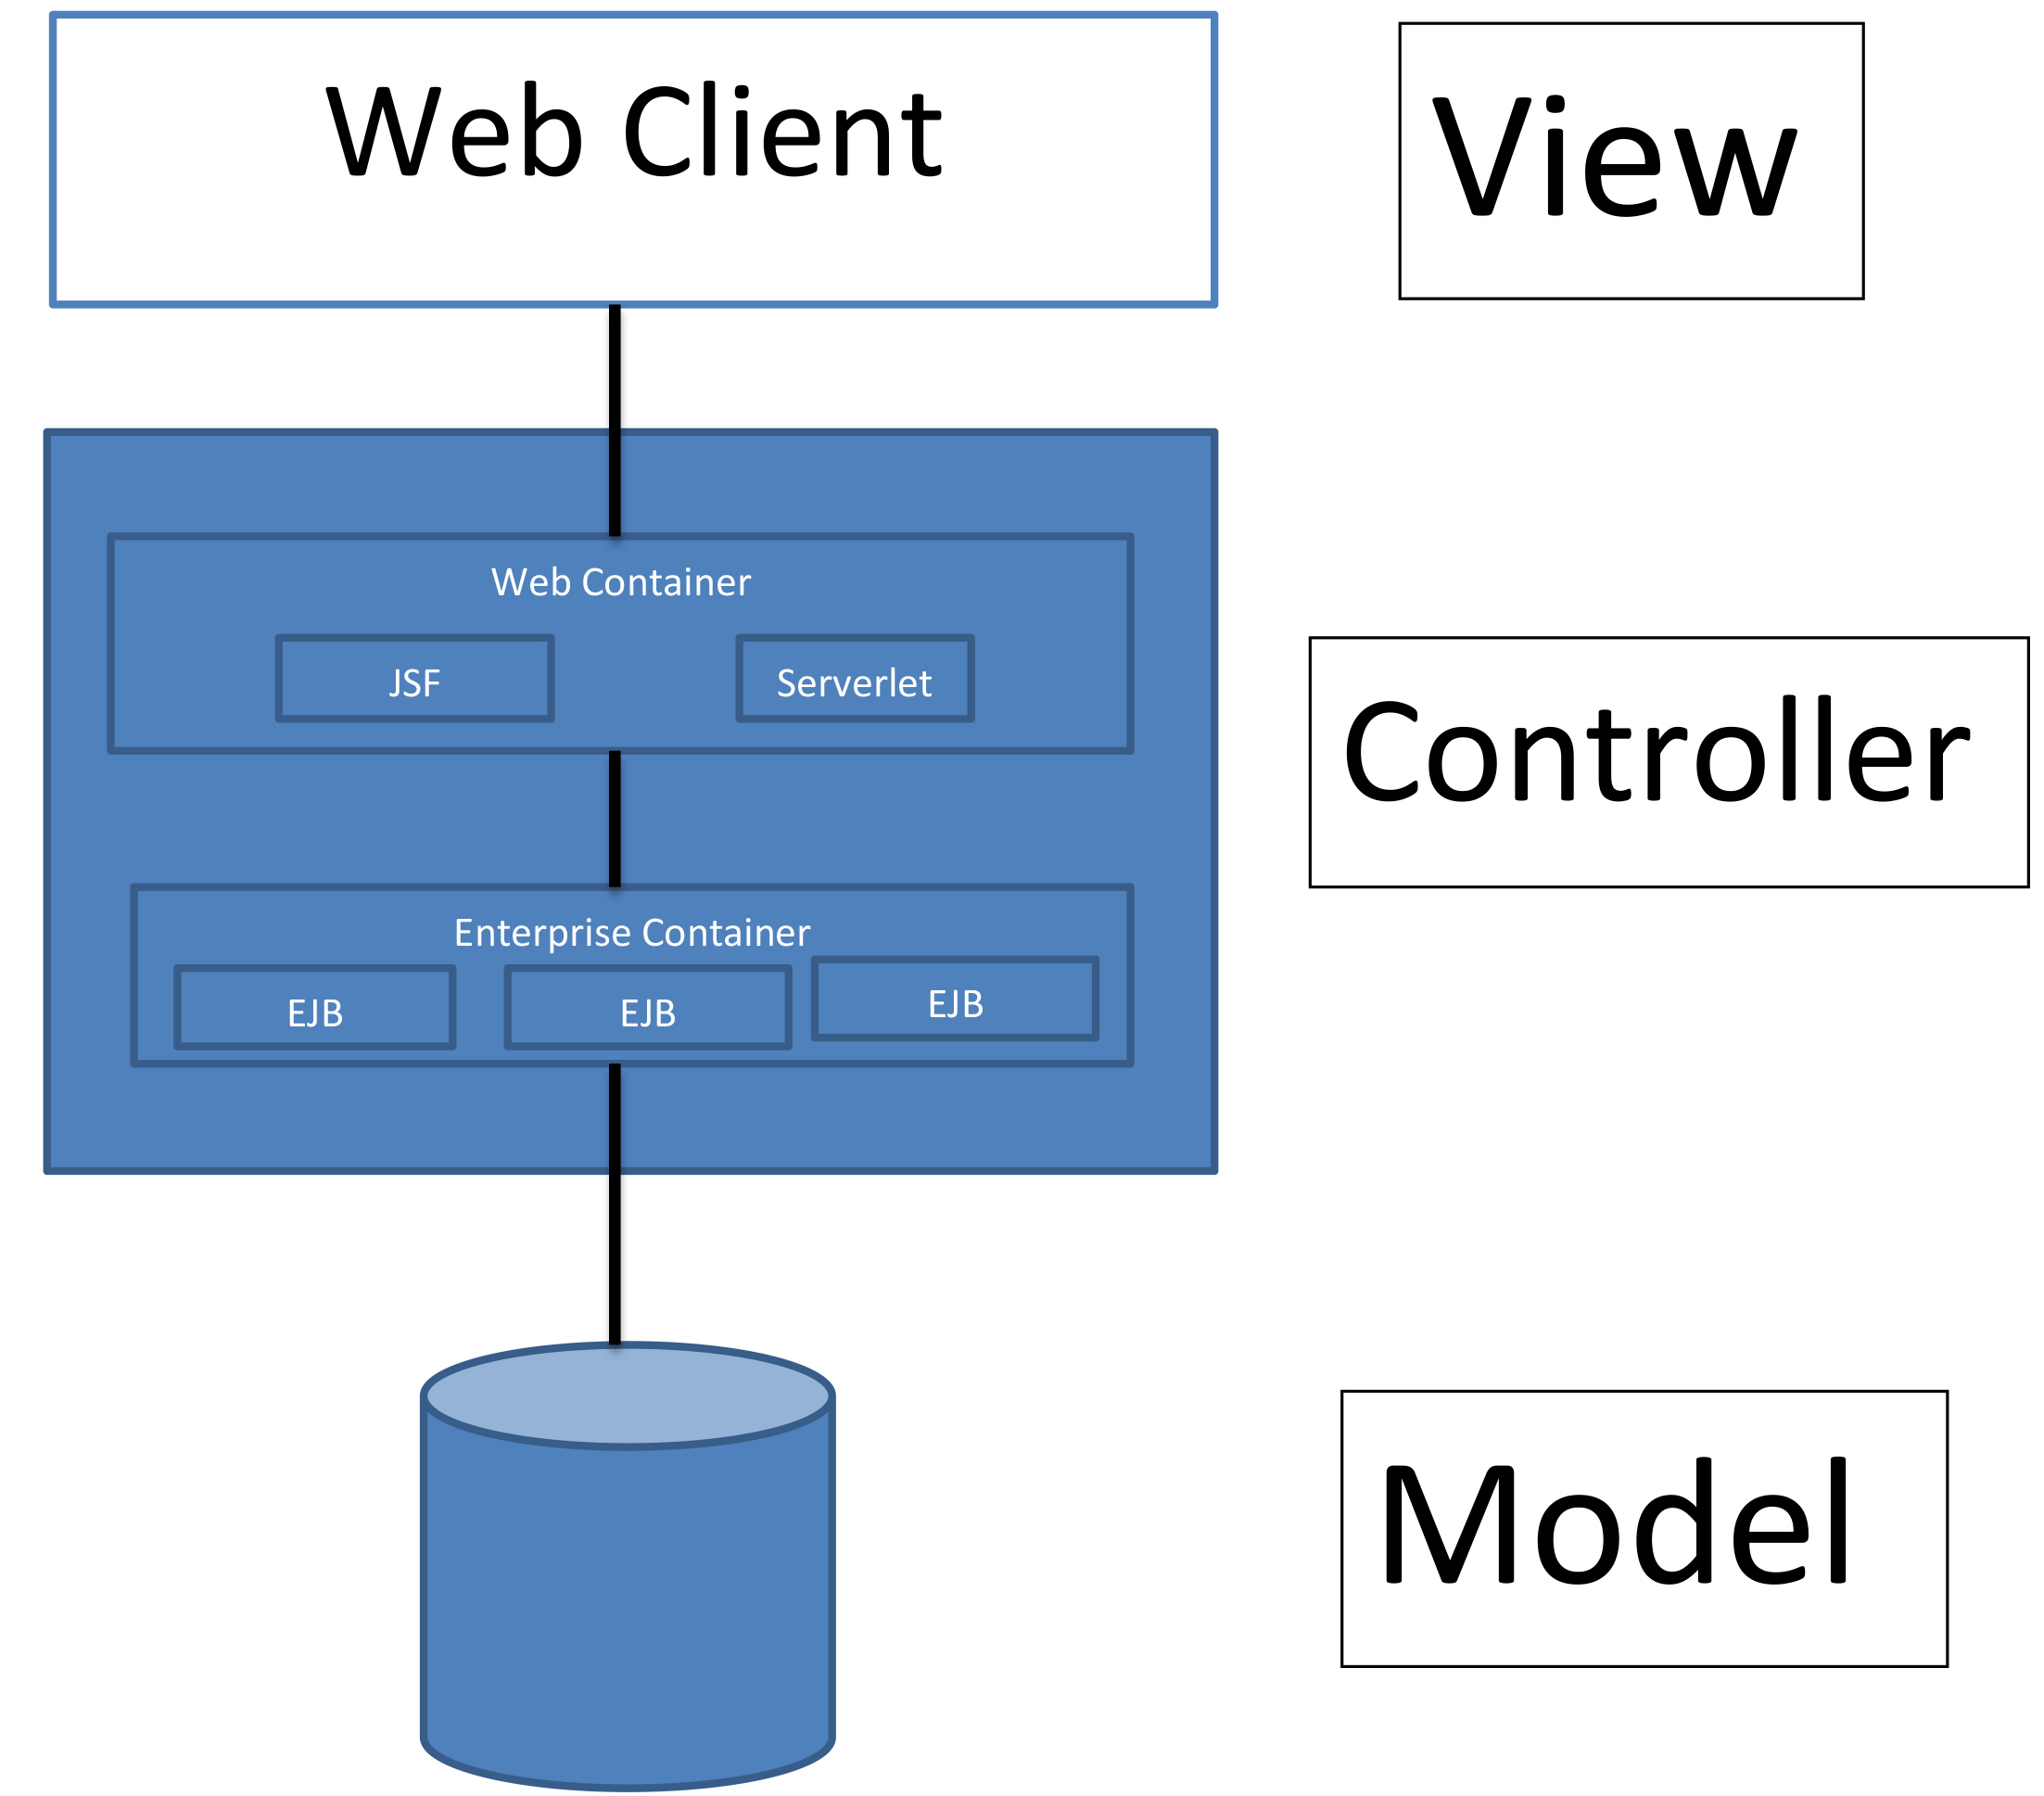
\includegraphics[scale=0.2]{../Images_Docs/Diagrams/Architecture/MVC.jpg}
\caption{Model View Controller of Architecture}
\end{figure}

\subsection*{View}
This component provides an interface to the under laying system to the user. This client is the web browser. It also incorporates components which are in the Web container(controller), such as Java Sever Faces. 
\subsection*{Controller}
This component is made up of two containers, the web container and the Enterprise container.
% More bullshit goes here.
\subsection*{Model}
This component is the actual database on which the system runs on. Which will be used as the centralised point of access with regards to applications being processed by the system as required by \client .
 
%%%%%%%%%%%%%%%%%%%%%%%%%%%%%%%%%%%%%%%%%%%%%%%%%%%%%%%%%%%%%%%%%%%%%%%%%%%%%%%%%%%%%%%%%%%%%%%%%%%%%%%%%%%%%
\section{Architectural Tactics and Strategies} % skipped till further notice.
This section describes techniques which will be used to satisfy the quality requirements. It the time of printing this document no architectural tactics/strategies have been identified as the architectural patterns and styles should be sufficient to satisfy the requirements.

%%%%%%%%%%%%%%%%%%%%%%%%%%%%%%%%%%%%%%%%%%%%%%%%%%%%%%%%%%%%%%%%%%%%%%%%%%%%%%%%%%%%%%%%%%%%%%%%%%%%%%%%%%%%%
\section{Use of Reference Architecture and Framework}
Java EE provides an API and runtime environment for developing and running large-scale, multi-tiered, scalable, reliable, and secure network applications. It also provides an architecture for implementing services as
multitier applications that deliver the scalability, accessibility, and manageability needed by the system. This is reason to why it is ideal to use it in the development of the project.

%%%%%%%%%%%%%%%%%%%%%%%%%%%%%%%%%%%%%%%%%%%%%%%%%%%%%%%%%%%%%%%%%%%%%%%%%%%%%%%%%%%%%%%%%%%%%%%%%%%%%%%%%%%%%
\section{Access and Integration channels}
This section discusses the requirements for the channels through which the system can be accessed by humans and other systems. Also making mention about the integration channels which need to be followed. 

\subsection{Access Channels}
The system will be accessible by humans through the recent versions of the following browsers:
\begin{enumerate}
\item Mozilla Firefox,
\item Google Chrome,
\item Microsoft Internet Explorer
\item Apple Safari, and
\item Opera
\end{enumerate}
The mobile counterparts of the above mentioned browsers will also be catered for and so no other access channel (such as Android/Apple apps) is to be considered.
\subsection{Integration Channels}
Upon successful complementation the system must be integratedable with the University of Pretoria's PeopleSoft system. Therefore it is sensible to implement the system in Java EE as it is one of the many components that form part of the multiple tiers that build up  PeopleSoft. \\
\\
The use of build tools such as Maven will provide a central piece of information with regards to the projects build, reporting and documentation. This central point of information will assist in the integration phase since it is implemented through a standardised build approach which can come into play at a later time through the use of EAI.\\
\\
The EAI will be achieved via  the logical integration architecture of Direct point-to-point integration. This means that the application management system will make direct JDBC calls to the universities databases tables (which needed to be setup to cater for our system at that point). The Integration method will be pushed-based data-level integration (or if all else fails UI-Level integration).
% http://www.javaworld.com/article/2074488/enterprise-java/enterprise-application-integration-using-j2ee.html

\section{Technologies}
The System will use the following technologies:
\begin{itemize}
\item Java Enterprise Edition 7
\item MySQL database
\item Netbeans 8.0
\item Glassfish server
\end{itemize}

\subsection*{Integrated Development Environment}
The system should be buildable independent of an IDE but it will be developed on Netbeans 8.0 to allow for uniformity amongst the development team, with regards to coding style, and provide easy integration with the tools that will be used such as Javadoc, to generate  API documentation in HTML format.

\subsection*{API}
\begin{itemize}
\item JavaMail
\item JavaBeans Activation Framework
% The JavaBeans Activation Framework (JAF) is used by the JavaMail API. JAF provides standard services to determine the type of an arbitrary piece of data, encapsulate access to it, discover the operations available on it, and create the appropriate JavaBeans component to perform those operations.
\item Java Database Connectivity
%The Java Database Connectivity (JDBC) API lets you invoke SQL commands from Java programming language methods. You use the JDBC API in an enterprise bean when you have a session bean access the database. You can also use the JDBC API from a servlet or a JSP page to access the database directly without going through an enterprise bean.
\item Java Naming and Directory Interface
\item Java API for XML Web Services
\item SOAP with Attachments API for Java
\item Java Authentication and Authorization Service
\end{itemize}

\subsection*{Build Tools}
\begin{itemize}
\item Apache Maven (for reasons explained in the integration channels section).
\end{itemize}

\subsection*{Operating System}
The system will be deployable on:
\begin{itemize}
\item Windows 7 and 8.
\item Linux based operating systems (specifically Kububuntu 13).
\end{itemize}
\newpage

\section{Glossary:} %Mathys
\vspace{0.2in}

\begin{itemize}

\item \textbf{API} - Application Programming Interface
\item \textbf{Application} -Both renewal applications or new fellowship applications are seen as applications by this project.
\item \textbf{CV} - Curriculum Vita
\item \textbf{EAI} - Enterprise Application Integration
\item \textbf{HTML} - Hyper Text Mark-up Language
\item \textbf{Java EE} - Java Enterprise Edition
\item \textbf{JDBC} - Java Database Connection
\item \textbf{MVC} - Model View Controller
\item \textbf{UI} - User Interface
\item \textbf{UP} - University of Pretoria
 
\end{itemize}	

\end{document}